\begin{frame}[ctb!]
\frametitle{Clay GDSM Degradation Rate Sensitivity}

Highly soluble and non-sorbing $^{129}I$ demonstrates a direct proportionality between dose rate and 
fractional degradation rate until a turnover where other natural system 
parameters dampen transport. Highly soluble and non-sorbing $^{129}I$ demonstrates a direct 
proportionality to the inventory multiplier.

\begin{figure}[ht!]
\begin{minipage}[b]{0.45\linewidth}
\centering
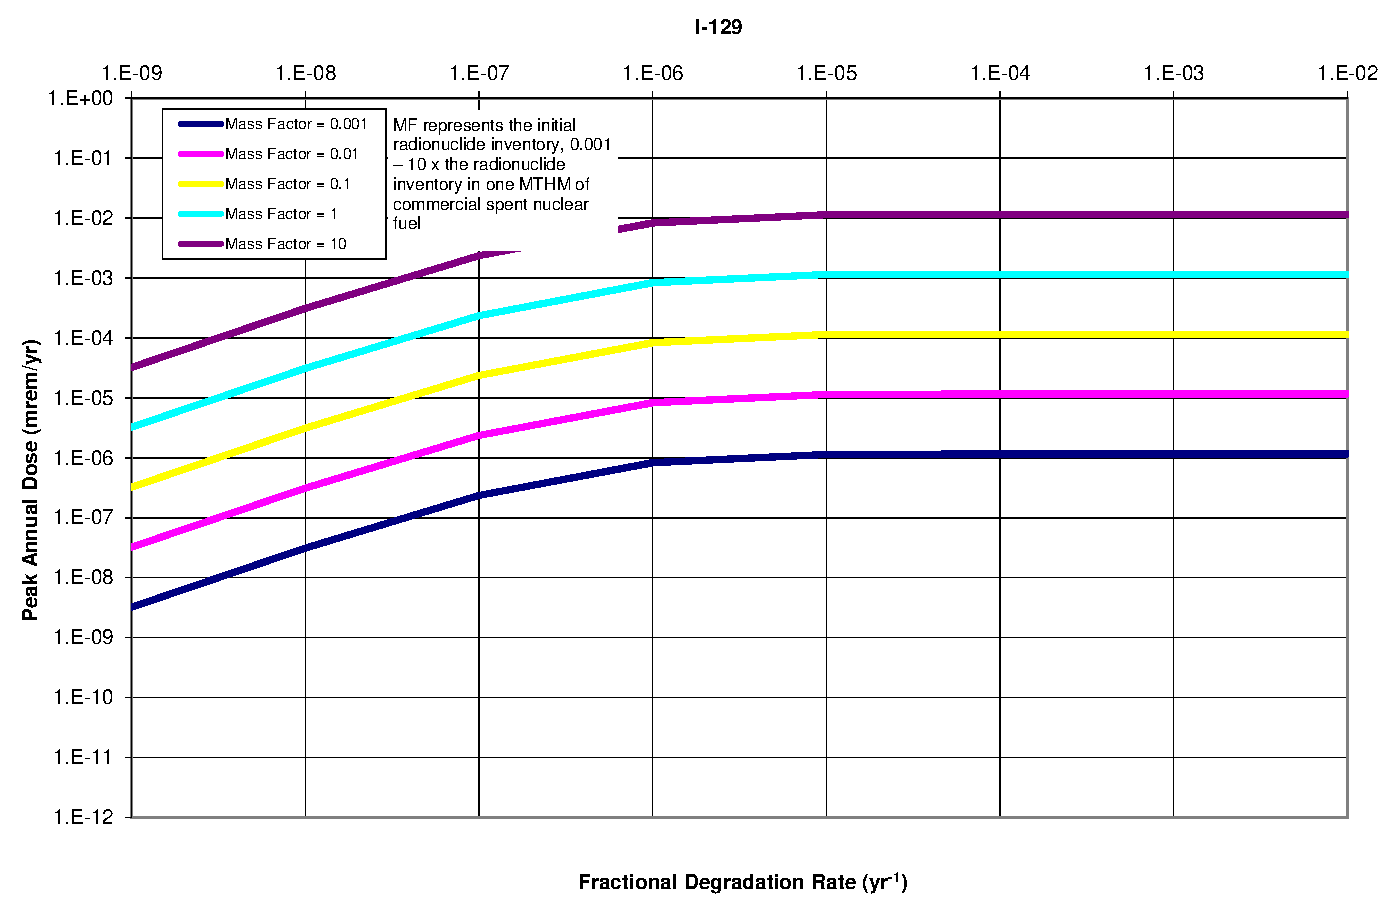
\includegraphics[width=\linewidth]{./nuclide_demonstration/DegRate/I-129.eps}
\caption{$^{129}I$ waste form degradation rate sensitivity.}
\label{fig:WFDegI129}

\end{minipage}
\hspace{0.05\linewidth}
\begin{minipage}[b]{0.45\linewidth}

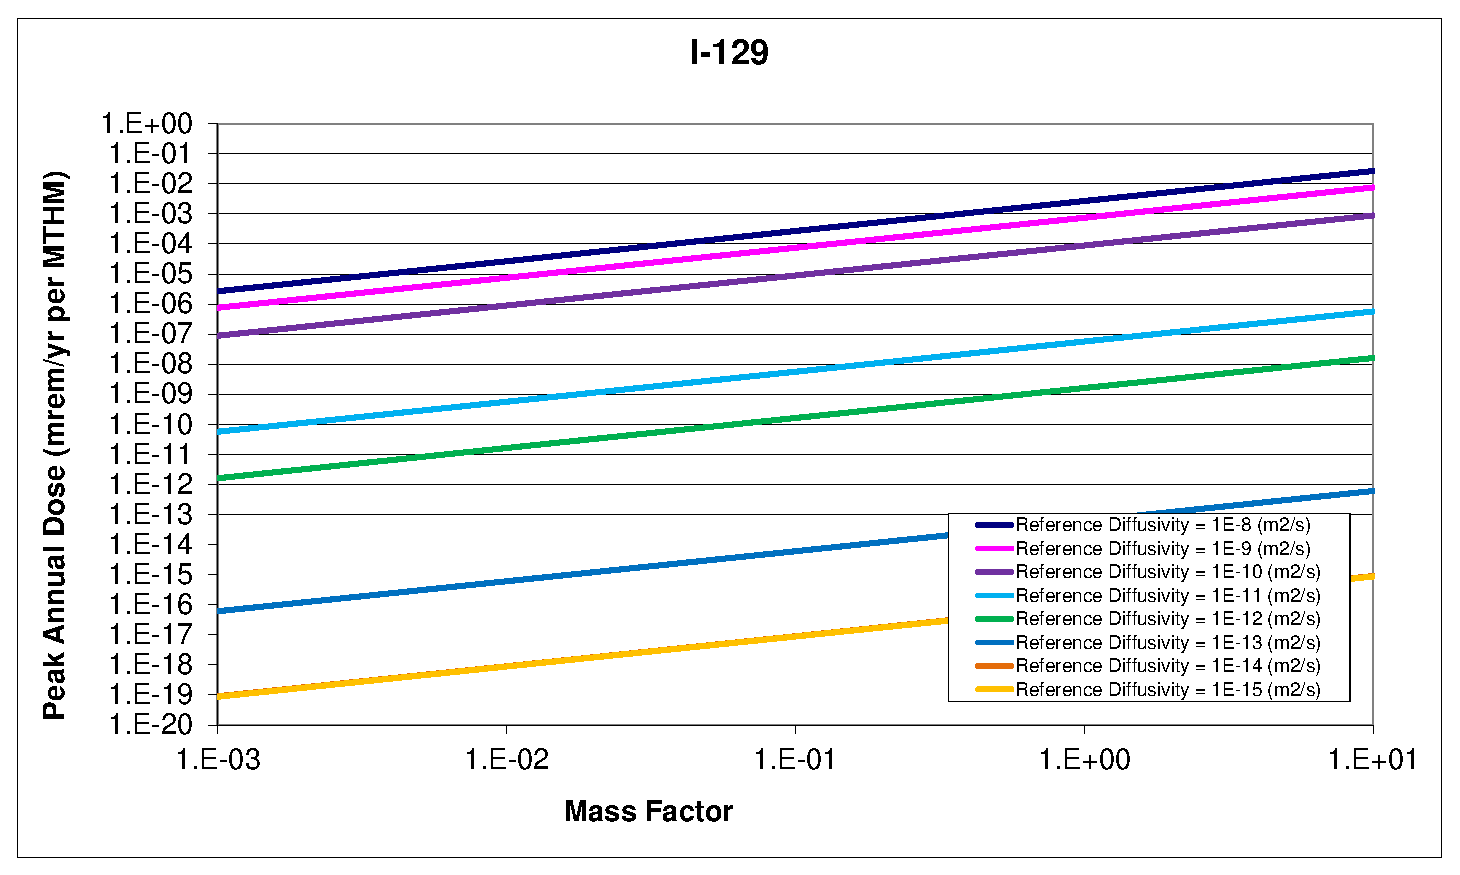
\includegraphics[width=\linewidth]{./nuclide_demonstration/DegRate/I-129-MF.eps}
\caption{$^{129}I$ inventory multiplier sensitivity.}
\label{fig:WFDegI129MF}

\end{minipage}
\end{figure}
\end{frame}
